\documentclass[a4,german]{article}

\usepackage[german]{babel} % für deutsche Silbentrennung und generierte Texte
\usepackage[T1]{fontenc}    % für deutsche Umlaute etc. in der Ausgabe
\usepackage[utf8]{inputenc} % für deutsche Umlaute.
\usepackage{graphicx}       % um Bilder einzubinden
\usepackage{hyperref}       % um URLs korrekt einzubinden und Hyperlinks im Dokument zu ermöglichen


\begin{document}

\title{Klassifikation von Wolkenarten: Ein Vergleich von verschiedenen Merkmalen zu CNNs} % TODO
\author{Maximilian Birkenhagen, Ali Ebrahimi, Thilo Fryen, Lukas Hintze} % TODO: Alles richtig geschrieben?
\maketitle % setzt automatisch den angegebenen Autor und Titel, sowie das heutige Datum als Überschirft (weitere Angaben möglich)


\begin{abstract}
    % TODO
    Wir klassifizieren Wolken...
    % vll erst schreiben, wenn der Bericht fertig ist
\end{abstract}

\newpage
\section{Einleitung}

% TODO: Einleitung
%Hier sollte stehen, was under Thema ist, warum es interessant ist, was andere Leute davor schon gemacht haben,
%was unsere Aufgabe ist, und wie unsere Arbeit aufgebaut ist.---

Wir haben uns dafür entschieden, Wolken zu klassifizieren; einerseits aus Neugier, wie gut dies möglich ist, und andererseits einfach aus eigenem Interesse an Wolken.

 Die Klassifikation von Wolken ist aber nicht nur für Wolken-Enthusiasten interessant, sondern spielt auch eine große Rolle bei der Klimaforschung, Wettervorhersagen und Unwetterwarnungen. Allerdings werden dabei eher andere Messmethoden wie Radar, Laser (z.B. LiDAR) oder Radiometer verwendet, bei denen Messungen von Sensoren an verschiedenen Orten (Satellit, Bodenstationen) kombiniert werden \footnote{Whang, Zhien; Sassen, Kenneth: Cloud Type and Macrophysical Property Retrieval Using Multiple Remote Sensors, University of Utah, 2001 - DOI:https://doi.org/10.1175/1520-0450(2001)040<1665:CTAMPR>2.0.CO;2}. Es gab aber auch schon versuche, nur mit Hilfe von Bildern Wolken zu klassifizieren: Forscher der Universität Kiel fotografierten den gesamten Himmel immer wieder von einer Position aus und unterschieden sieben verschiedene Wolkenarten(kombinationen), darunter auch "leerer Himmel". Mithilfe eines k-nearest-neighbour Klassifikators erreichten sie bei der Leave-One-Out Cross-Validation eine Genauigkeit von 97\% \footnote{Heinle, A.; Macke, A.; Srivastav, A.: Automatic cloud classification of whole sky images, Universität Kiel, 2010 - DOI: 10.5194/amt-3-557-2010}.

Unsere Aufgabe war es, Wolken einerseits mit dem 'klassischen' Ansatz und andererseits mittels Convolutional Neural Networks (CNN) zu klassifizieren und die Ergebnisse zu vergleichen. 
Für die Klassifizierung mit dem 'klassischen' Ansatz haben wir verschiedene Merkmale, wie zum Beispiel: Mittelwert, Standabweichung, Farb-Histogramm und Kantenerkennung verwendet.
 
 Dieser Bericht ist so aufgebaut, dass wir erst erklären wo unsere Bilder herkommen, was für Charakteristika sie haben und wie wir diese verarbeitet haben. Danach wird unsere Methodik erläutert, wie wir Probleme gelöst haben und was für Verfahren wir angewendet haben. Sodass zum Schluss ein aussagekräftiges Fazit mit Hinsicht auf unsere Ergebnisse gezogen wurde.
 
Entstanden ist diese Ausarbeitung im Rahmen des Praktikums 'Computervision' an der Universität Hamburg im Sommersemster 2018.



\section{Daten}

% TODO: Daten
%Hier sollte stehen, woher unsere Daten kommen, wie sie aussehen, was für Charakteristika sie haben, und was so klassentypische Einträge sind.

Unsere Bilder haben wir von der Website Wolken-online.de und von der World Meteorological Organization (WMO).
Insgesamt standen uns ca. 800 Bilder zur Verfügung.
Die Bilder waren meist von individuellen Personen geschossene Bilder vom Himmel. 
Allerdings ist auf den Bildern oft nicht nur der Himmel zu sehen, sondern auch am unteren Rand die Erde, zum Beispiel Häuser oder Bäume. Außerdem sind gelegentlich mehrere Wolkenarten auf dem selben Bild vertreten.

Der \textit{International Cloud Atlas} unterscheidet zehn Wolkengattungen, welche in Abbildung 1 schematisch dargestellt sind. Da diese sich untereinander teilweise sehr ähneln und wir lieber weniger Klassen unterscheiden wollen, haben wir diese in vier Hauptgruppen unterteilt.
\begin{itemize}
\item Cirriform: Cirrus
\item Cumuliform: Cumulus, Cumulonimbus
\item Stratiform: Cirrostratus, Altostratus, Numbostratus, Stratus
\item Stratocumuliform: Cirrocumulus, Altocumulus, Stratocumulus
\end{itemize}

\begin{figure}[h]
\centering
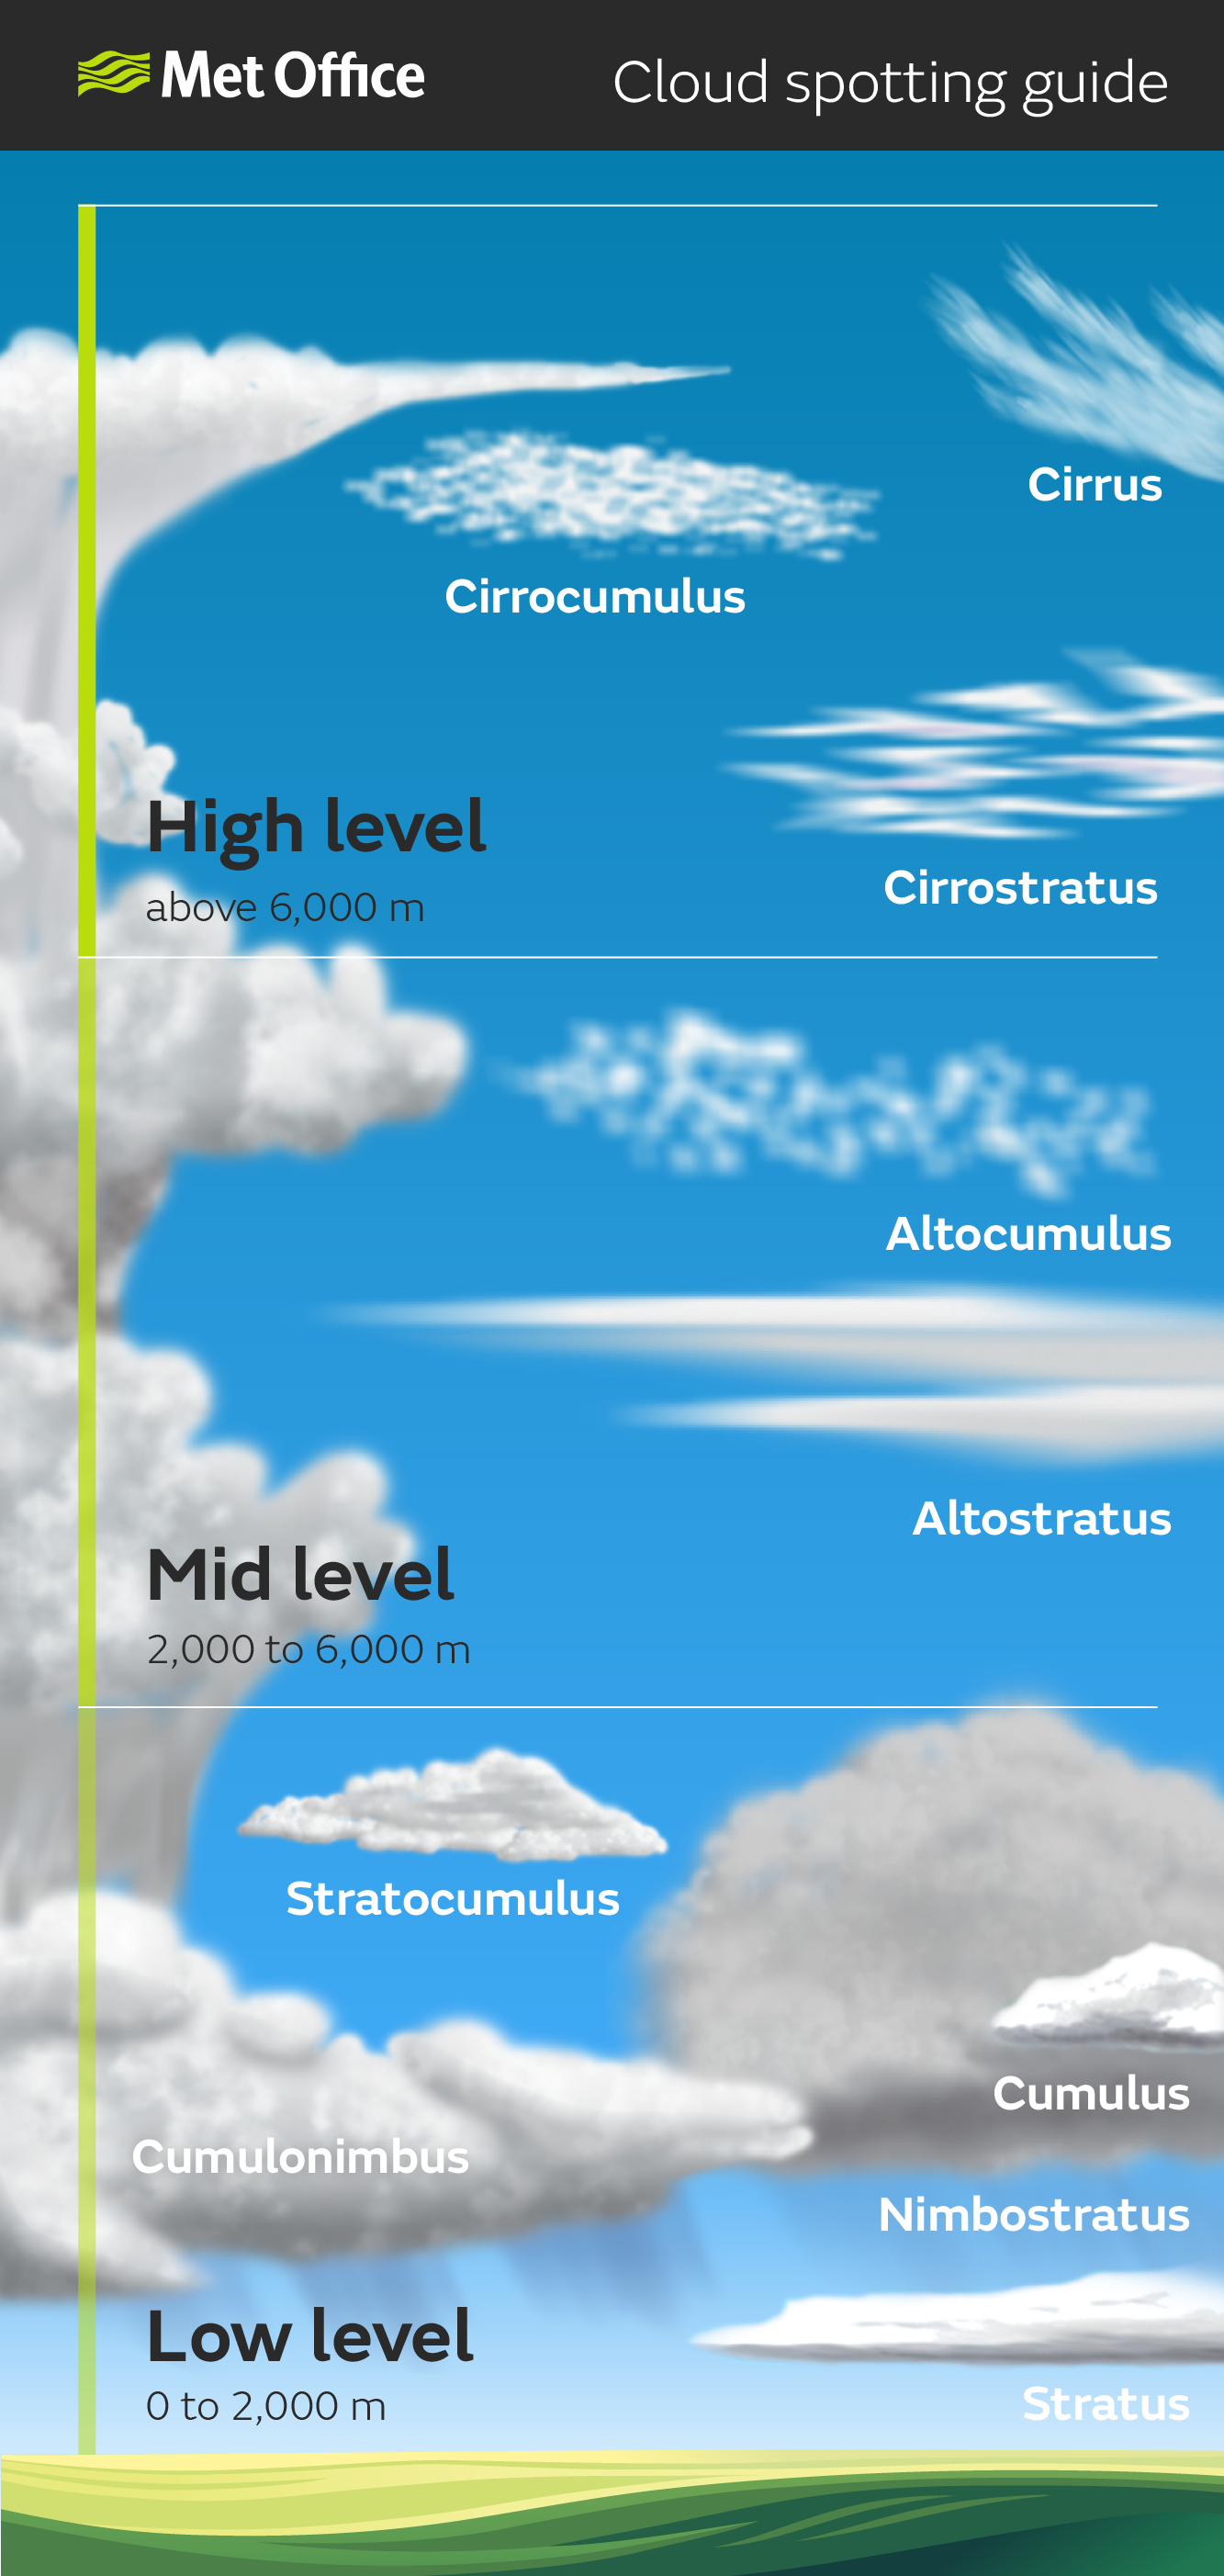
\includegraphics[width=10cm,height=14cm,keepaspectratio]{Cloud_infographic-01.png}
\caption{Schematische Darstellung der zehn Wolkengattungen}
    \label{fig:cloudtypes}
\end{figure}

Die Wolkenarten unterscheiden sich im wesentlichen durch ihre Struktur, Dichte und Höhe, wobei die letzten beiden auf Bildern nur schwer bis nicht erkennbar sind. Die stratiformen Wolken zeichnen sich dadurch aus, dass sie sehr flächig und zusammenhängend sind und meinst durchgängig den ganzen Himmel bedecken. Die cirriformen Wolken sind gefedert und oft durchsichtig, da sie sehr dünn und gefächert sind. Die cumuliformen Wolken haben die Form von großen Haufen, während die Stratocumuliformen Wolken die Form von vielen kleinen Haufen haben. Leider, wie man auch schon an den Namen der verschiedenen Wolkengattungen sieht, gehen sie ineinander über, was die Unterscheidung deutlich erschwert. Außerdem gibt es noch sehr viele, Arten, Unterarten und Begleitwolken, die sich teilweise auch überschneiden \footnote{Eine gute Übersicht der Wolkengattungen, -arten, etc. findet man unter\\ https://de.wikipedia.org/wiki/Wolke\#Übersicht, zuletzt aufgerufen im August 2018} . 

\section{Methodik}

% TODO: Methodik
%Hier sollte stehen, wie wir unser Problem lösen, sprich, wie unser Endsystem funktioniert.
%Warum machen wir es so und nicht anders?
%Wie funktionieren die Verfahren, die wir nutzen?
%Auch eine Ablaufgrafik wäre nice.

\subsection{Beschaffung der Bilder}

\subsection{Verwertung der Bilder}
Da die Bilder verschieden waren, mussten wir sie vor der Klassifikation anpassen.
Zuerst haben wir unpassende Bilder, wie zum Beispiel von einem Sturm oder Bilder, auf denen die Wolken kaum erkennbar waren, manuell aussortiert.
Wie erwähnt war oft der untere Rand des Bildes nicht mehr der Himmel, sondern zum Beispiel eine Wiese oder Bäume.
Durch eine Binarisierung konnten wir relativ akkurat den Himmel ausschneiden.
Zum Schluss haben wir die Bilder noch auf die Einheitliche Größe von 500x500 Pixel gebracht, bei welcher die Algorithmen noch schnell ein genaues Ergebnis berechnen konnten. 

\subsubsection{Binarisierung}
Die Binarisierung haben wir mithilfe des arithmetischen Mittels des gesamten Bildes und dem Hue + Value aus dem HSV-Farbraum implementiert.
...
Hier Boxalg erklären
\subsection{Augmentation der Bilder}




\section{Experimente und Ergebnisse}

% TODO: Fazit
%Wie sehen unsere Ergebnisse aus?
%Wie verändern sich die Ergebnisse durch die CNNs?
%Was passiert, wenn man einzelne Teile des Systems austauscht oder Merkmale entfernt (dies evtl.\ auch mit Diagrammen zeigen)?
%Wie schneidet das System pro Klasse ab?
%Wie wirken sich Änderungen der Parameter/Hyperpara\-meter auf die Ergebnisse aus?
%Wie schnell sind unsere Verfahren?


\section{Fazit}

% TODO: Fazit
%Was ist unser Fazit?
%Zusammenfassung und Einordnung unserer Ergebnisse.
%Ausblick?


% Literaturverzeichnis mit Hilfe der "thebibliography" Umgebung:

\begin{thebibliography}{99}
	
% Beispiel für ein Buch
\bibitem {mustermann1234} M. Mustermann. \textit{Das hier ist nur ein Beispiel}. Musterverlag, 1234.

\end{thebibliography}



\end{document}
